\documentclass[9pt,twocolumn,twoside]{../../styles/osajnl}
\usepackage{fancyvrb}
\journal{i524} 

\title{Google Cloud storage: A journey towards Cloud storage}

\author{Kumar Satyam}

\affil[1]{School of Informatics and Computing, Bloomington, IN 47408, U.S.A.}

\affil[*]{Corresponding authors: ksatyam@indiana.edu}

\dates{paper-1, \today}

\ociscodes{Cloud,Google Cloud Storage, BigQuery, Buckets, Objects, I524}

% replace this with your url in github/gitlab
\doi{\url{https://github.com/satyamsah/sp17-i524/blob/master/paper1/S17-IR-2031/report.pdf}}


\begin{abstract}
 Now-a-days due to exponential growth of data, it is almost impossible to store the huge amount the data locally in our own systems or local storage boxes which are prone to data loss in case of hardware failure. With cloud storge one can save the data in cloud without any risk of data loss because of redundacy of data over cloud.It explains about the Google cloud storage technology which is one of cloud storage vendor.We will discuss what are the key elements of Google cloud storage and try to relate it with the general cloud storage technology\cite{www-scientific-paper}.
 
\hfill \break
\end{abstract}

\setboolean{displaycopyright}{true}

\begin{document}

\maketitle


\section{Introduction}

Google cloud storage is a unified object storage mainly targeting enterprises and developers which offers capability of both live data serving with high I/O throughput to data archiving. 
As shown in Fig \ref{fig:arch}, it is a RESTful online file storage web service for accessing data on Google Cloud platform \cite{www-google-cloud-storage-wiki}. It is an IAAS cloud delivery model which provides good performance and scalability using Google's cloud platform. 


\begin{figure}[htbp]


\section{Architecture -Google Cloud Platform}

\hfill \break
\centering
\fbox{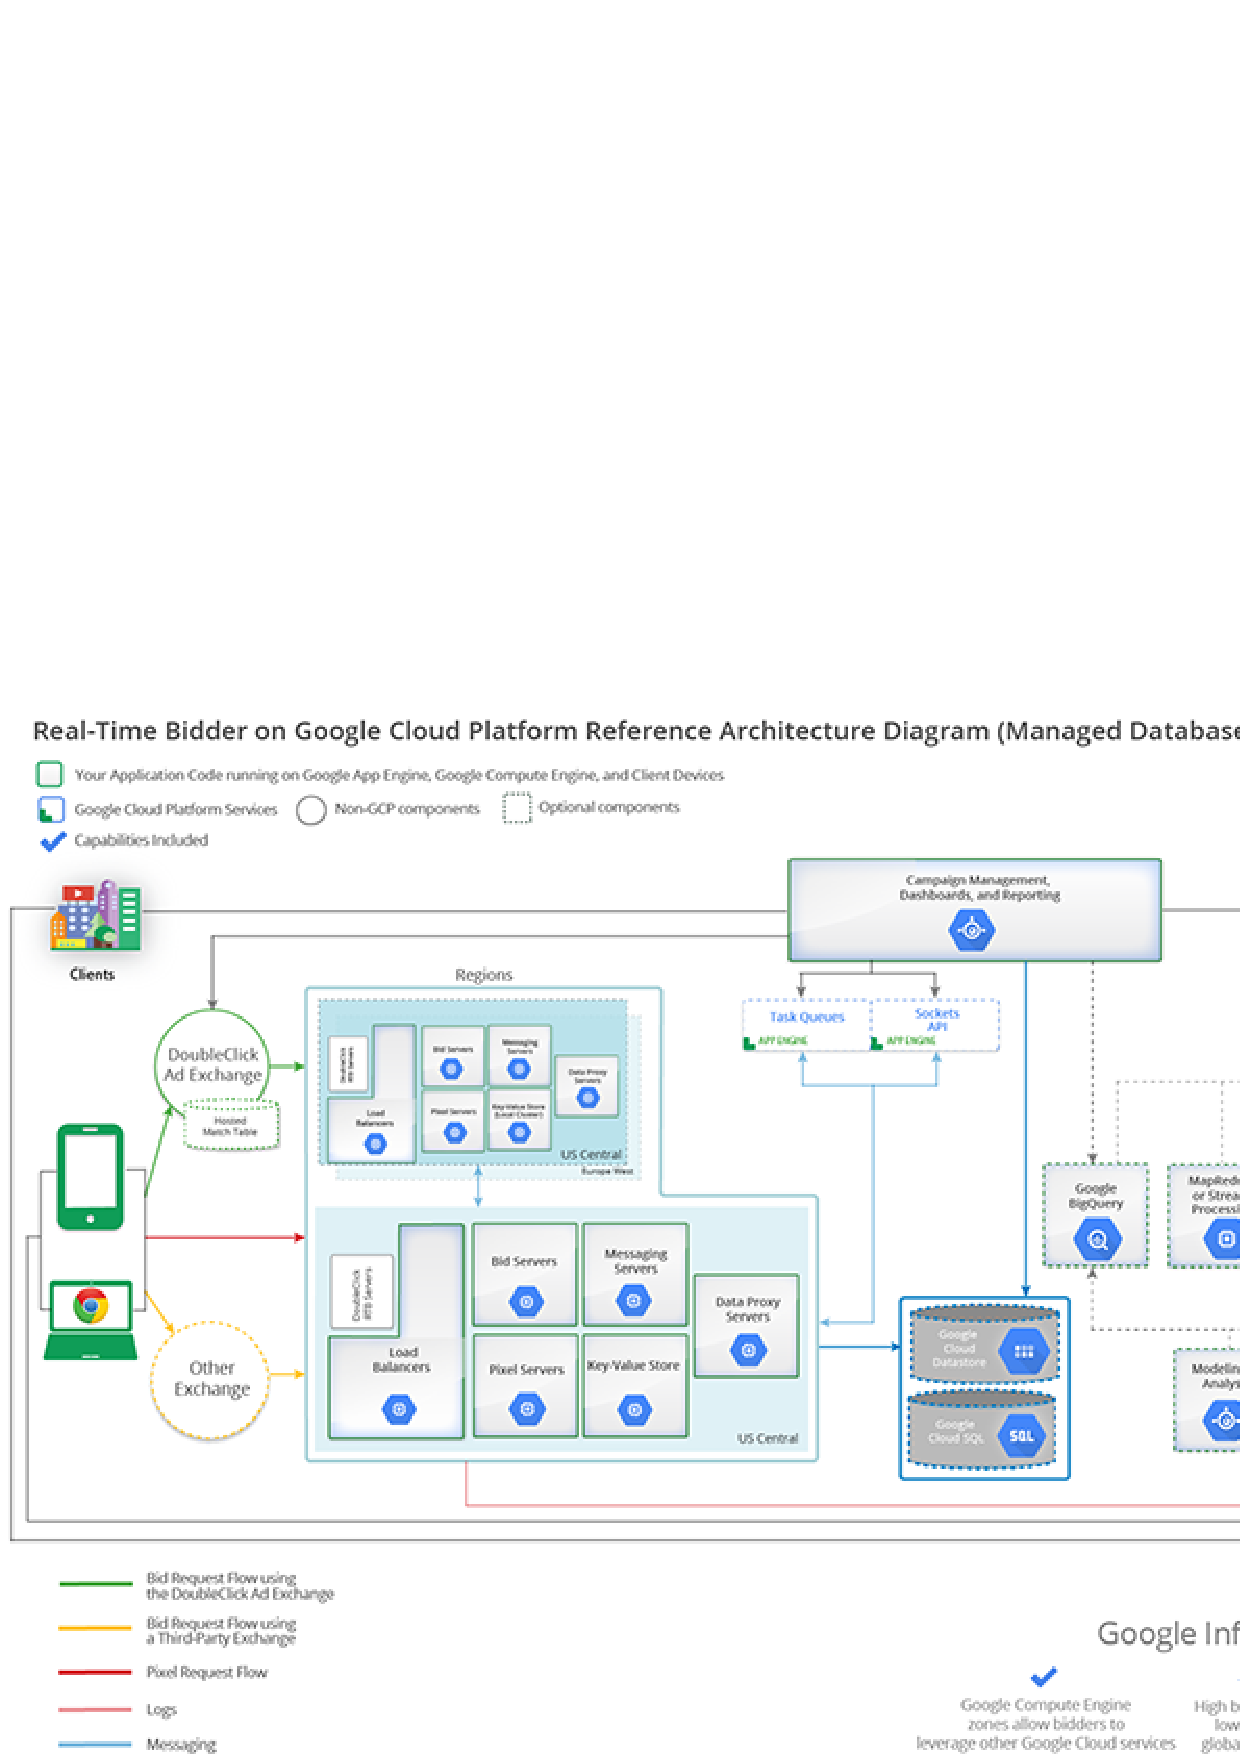
\includegraphics[width=\linewidth]{images/sample}}
\caption{Architecture of Google cloud platform using Google cloud storage as persistent layer \cite{www-google-cloud-storage}  }
\label{fig:arch}

\end{figure}


\section{Key Terms}

\begin{flushleft}

Projects: 

All the data in Google Cloud storage belongs inside a project. A project consists of	 a set of users, set of API and billing, authentication and monitoring setting for those APIs.\cite{www-google-cloud-storage} 
\end{flushleft}


\begin{flushleft}
Buckets:

Buckets are basic containers that hold the data. Everything that a user/organization stores in Google Cloud Storage must be contained in a bucket. Buckets have bucket name. In Google cloud storage, buckets are created to store the data. A Bucket has three properties,a location is where the bucket and its contents are stored, a globally unique name and, a default storage class.For example, if a user specify the location 'eu'(European union)  when he creates a bucket A, then bucket A and any objects of bucket A are stored on servers of European union region. 

\end{flushleft}


\begin{flushleft}

Objects:

Objects are individual pieces of data which are stored in Google cloud storage. A single object can go up to 5 TB in size. Objects have 2 components: Object data and object metadata. The object data component is usually a file that a user to store in Google cloud storage.
Object name is just meta data to cloud storage. A common character in the file system is the slash (/). By slash an object name appear as they are stored in hierarchical structure. But Google cloud storage sees the object as independent objects with no hierarchy.
\end{flushleft}


\begin{flushleft}

Data opacity: 

An Object’s data component is completely opaque to Google cloud storage. It is just a chunk of data to Google Cloud storage.

\end{flushleft}


\begin{flushleft}
Object immutability: 

Objects are immutable which means that an object cannot change throughout their storage lifetime. An object's storage life time is between the successful object creation and successful object deletion. 
\end{flushleft}


\begin{flushleft}
Hierarchy:

Google cloud storage uses a flat namespace to store objects. However, some tools show it in hierarchical manner.
\end{flushleft}


\begin{flushleft}
Namespace:

There is only one google cloud storage namespace that means every bucket should have a unique name. Object name must be unique inside a bucket.
\end{flushleft}


\section{storage classes}

In Google cloud storage bucket is the place where a user can store data.As explained earlier bucket needs be in a 'Storage class'. One can think this a service tiers of creating a bucket.There are 4 storage classes offered in cloud cloud storage:



\begin{flushleft}

Multi-regional storage:

This offers 99.95 \% availability with geo-redundant feature. It provides maximum availability of the data even in case of large scale disruption. It is used to store data that is frequently access around the world, such as serving website content. The cost of using this storage class is \$0.026 per GB per month. Till now there are three multi – region location 
		\begin{itemize}

			\item asia — Asia Pacific
			\item eu — European Union
			\item us — United States

		\end{itemize}
\end{flushleft}


\begin{flushleft}
Regional storage:

It is used for high availability and redundancy within a single region. This offers 99.95 \% availability. The cost of using this storage class is \$0.02 per GB per month. It is recommended to the users to use “Regional”  storage to utilize durable  reduced  availability. A user can move data from DRA to other storage classes by performing a storage transfer. It is best when a user wants to optimized latency, availability and, network bandwidth within the same location. It can still be read globally , but if the organization's bucket is used primarily by client outside region , it is better to switch to multi-region location.It is best for application which require high data analysis and computation.Till now there are three multi–region location :

		\begin{itemize}

			\item asia-east1 — Eastern Asia-Pacific
			\item asia-northeast1 — Northeastern Asia-Pacific
			\item europe-west1 — Western Europe
			\item us-central1 — Central United States
			\item us-east1 — Eastern United States
			\item us-west1 — Western United States

		\end{itemize}
\end{flushleft}


\begin{flushleft}
 Nearline Storage:

It is a storage offering which is suited for the archived data which the user access less than once a month .It is low cost, highly durable storage service for infrequently accessed data. It is ideal for back-up and serving long-tail multimedia. The cost of using it is \$ 0.01 per GB per month. 

\end{flushleft}


\begin{flushleft}
 Coldline storage:

Coldline storage is the storage which is used for the data which the user access less than once a year. Typically this used in case of disaster recovery where it provides low latency to access  data stored in Coldline storage ,or for the data that is archived and may or may not be needed at some future time. Cost is using this \$  0.007 per GB per month.


\end{flushleft}


\begin{flushleft}
 Standard storage: 

When a user creates a bucket without specifying storage class, the cloud storage  will create a standard bucket which can be either be a multi-regional or a regional storage based on the location the user is creating the storage bucket. If a user has a standard storage in a multi-regional location like ‘us’ then it is equivalent to multi regional storage and continue to exist in ‘us’ location. If the standard storage is in the regional storage like ‘us-east’, it will be equivalent to ‘regional’ storage 

\end{flushleft}


\begin{flushleft}
 Note:
Each bucket has a default storage class which one can specify while creating the bucket. The objects also take the default storage unless specified otherwise. One can change the default storage class of  his bucket anytime. But the objects which were created in the bucket before changing the storage class will remain in the same(earlier) storage class and will not change to new storage class. It will only affect the storage class of the objects which will be created after the change of the storage class of the bucket.
One can specify the storage class of each object which is added to the bucket or can change their name afterwards using the API calls. 

\end{flushleft}



\section{Access Control Options}

This takes care of authentication and authorization mechanism. One can control who has access to organization's Cloud storage buckets and objects as well as what level of access they have. 



\begin{flushleft}
Identity and access management(IAM):

IAM grants access to project's bucket and objects.For example, one can specify that a user has full control of all the objects in an organization's projects, but cannot create, modify, or delete any buckets in the projects. IAM gives broad control over the project but not fine-grained control over individual buckets or projects.
\end{flushleft}


\begin{flushleft}
Access control list:

 It is authorization mechanism of Google cloud storage in which read or write access is granted to users for individual buckets or objects.

\end{flushleft}


\begin{flushleft}
Signed URLs:
 
These URLs give time limited read-write access to an object through a URL the owner can generate. This can be generated using "gsutil" or by a program. The owner only need to share the url and recipient can access the object through the URL for a specific duration of time which the owner specifies.

\end{flushleft}


\begin{flushleft}
Signed Policy Document:

This is a document which Specify the type,size and, other upload characteristics of data which can be uploaded and can be used by website owner to allow visitors to upload files to Google file storage
\end{flushleft}



\section{Google Cloud Platform Console }

One can use Google cloud Platform Console to perform simple storage management tasks for cloud storage.It requires only a browser to work. Some of the task include:
- Enable the Google Cloud storage API for a project
- Creating and deleting buckets 
-Uploading, downloading and deleting objects
- Managing ACLs for objects and buckets.


One can use other methods like using the "gsutil" command line tool or any of the client library that supports Google Cloud Storage.

\subsection{Accessing Google Cloud Platform Console}


Google Cloud Platform Console requires no setup or installation and one can access it directly through a browser. There are different ways to access cloud platform console depending on the type of user:




\begin{flushleft} 
A project member: 

In order to use Google Cloud Platform Console as a project member, the person account must be added to the list. A current project owner can give the person account privileges like owner, editor, or viewer access to the project which applies to all the buckets defined in the project.
\end{flushleft}


\begin{flushleft}
 A user granted read or write access to a bucket:

In this case , a project owner  gives a user read or write access to a bucket name.This is useful for the people who are not the project member but need to access the bucket.This URL will prompt the user to authenticate with a Google account if the user is not already signed in.
	
\end{flushleft}


\begin{flushleft}
A user is granted read access to an object:

In this case the project owner configures an object as publicly viewable and sends the user the URL to access the object. This URL will prompt the user to authenticate with a Google account if he are not already signed in.This is different from the process of "sharing the URL publicly". In the option of "sharing the URL publicly" the URL does not need any authentication.

\end{flushleft}




\subsection{Using the Google Cloud Platform Console to Manage the Data}

An owner can perform various actions which can be performed while accessing Google Cloud storage using console.

\begin{itemize}


\item To create a bucket
\item Uploading data to a bucket
\item Downloading data from a bucket
\item Creating and using folders
\item Deleting objects, folders, and buckets
\item Sharing the data publicly
\item Setting bucket permissions
\item Setting object permissions and metadata
\item Filtering objects to view
\item Adding a member to a project

\end{itemize} 

\section{Google Cloud storage in Bigdata}

Google cloud platform and google cloud storage is apt to handle massive tasks working on both the structured and unstructured way.Analytics and machine intelligence at web-scale have been used to solve data intensive tasks.Google BigQuery \cite{www-google-bigquery} is cloud platform's  managed data warehouse that lets an organization economically query massive volumes. It is ideal to run Spark and Hadoop.

\section{Google Cloud storage competitors}
In the cloud platform business where all the market leader like AWS, Microsoft Azure, IBM Bluemix etc., Google cloud platform is also giving good competition.It is spreading its services by coming up with more regions and availability zones all across the world with cheap rates. 

\section{conclusion}
This paper has shown the key aspects of the cloud storage systems, how it works and how it is an integral part of the Google cloud platform,some core concepts of Google Cloud storage. It also showed how Google cloud storage performing with respect to Big data technology. And how it is performing in comparison to other vendors who are in the market.

\bibliography{references}

\end{document}
